% File project.tex
%% Style files for ACL 2021
\documentclass[11pt,a4paper]{article}
\usepackage[hyperref]{acl2021}
\usepackage{times}
\usepackage{booktabs}
\usepackage{todonotes}
\usepackage{latexsym}
\usepackage{multirow} 
\usepackage{xcolor}
\usepackage{graphicx}
\usepackage{hyperref}

\renewcommand{\UrlFont}{\ttfamily\small}

% This is not strictly necessary and may be commented out,
% but it will improve the layout of the manuscript,
% and will typically save some space.
\usepackage{microtype}

\aclfinalcopy 
% i\newcommand\BibTeX{B\textsc{ib}\TeX}

\title{Baselines and Analysis}

\author{
  Ming-Feng Li\thanks{\hspace{4pt}Everyone Contributed Equally -- Alphabetical order} \hspace{2em} Pujith Kachana$^*$ \hspace{2em} Shashwat Chawla$^*$ \hspace{2em} Yatharth Ahuja $^*$ \\
  \texttt{\{mingfenl, pkachana, shashwac, yahuja\}@andrew.cmu.edu}
  }

\date{}

\begin{document}
\maketitle

\section{Analysis of Baselines}

Our goal is to develop a robust Visual-LiDAR odometry system, comparing against various unimodal, multimodal, classical, and learning-based baselines. Our model uses optical flow for image representations and a LiDAR point map as input to a transformer with cross-attention for pose regression. This approach combines the strengths of visual methods (flow-based correspondences) and LiDAR methods (3D geometry) while drawing on classical odometry principles and multimodal fusion techniques.

Unfortunately, it is difficult and unhelpful to find unified intrinsic metrics across these various baselines. So, for each key baseline below, we discuss the key components we adapted to our model and report the relevant metrics for that baseline, along with our conclusions.

\subsection{Intrinsic Metrics}

\subsection{Visual Odometry Methods}

We assessed two visual odometry methods, one based on classical algorithms and the other on learning-based approaches. Their evaluations are presented in the following sub-sections.
\subsubsection{ORB-SLAM}
ORB-SLAM2 \cite{orb-slam2} is a powerful and versatile visual odometry system known for its robust performance across various camera setups, including monocular, stereo, and RGB-D cameras. It was evaluated as a classical unimodal (visual) odometry baseline due to its wide adoption and success.

The algorithm operates with three main components: tracking, local mapping, and loop closure. Tracking estimates camera pose in real-time, local mapping updates the map using keyframes and landmarks, and loop closure detects previously visited locations, reducing positional drift over long distances. Designed for efficiency, ORB-SLAM2 runs in real-time on standard CPUs, making it practical for real-world applications.

Key features of ORB-SLAM2 include robust loop closure capabilities that enhance long-term accuracy and adaptability to different environments. Its performance on the KITTI \cite{KITTI} odometry benchmark—a widely used dataset for outdoor visual odometry evaluation—demonstrates ORB-SLAM2's scalability and effectiveness, with an average translational error of 1.15\% and a rotational error of 0.0027 degrees per meter for stereo input. The system consistently performs well across sequences, showcasing its resilience to various environmental challenges and confirming its reliability for large-scale environments. Some interesting results of the interesting inference runs are shown in figure \ref{fig:orb-slam2}.

% The evaluations of ORB-SLAM2 on KITTI sequences are presented in Table \ref{tab:orb-slam2}. 


\begin{figure}[h!]
    \centering
    \subfigure[Sequence 02]{
        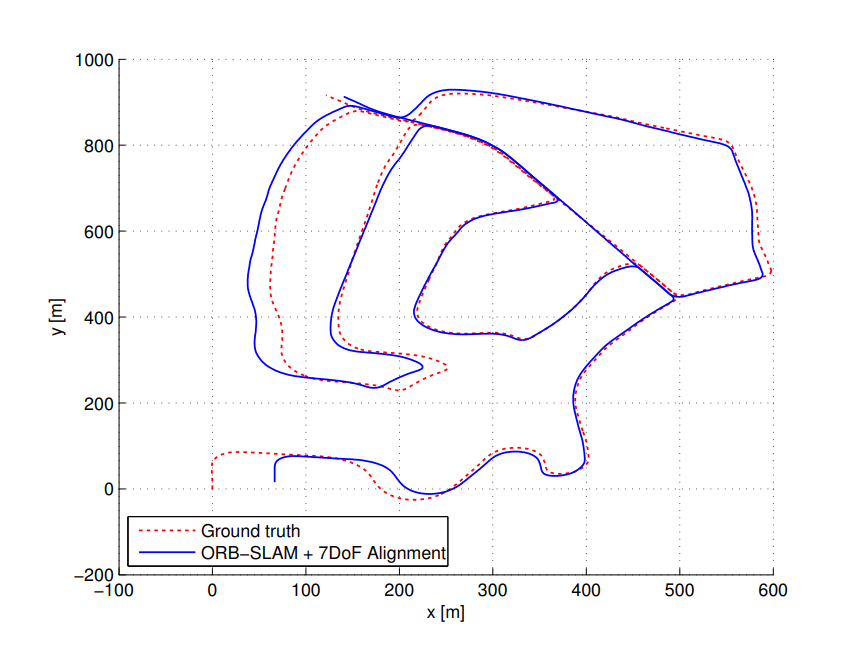
\includegraphics[width=0.4\textwidth]{Reports/3-Analysis-of-Baselines/images/orb02.png} % Replace with your image file
        \label{fig:orb-slam11}
    }
    \hspace{0.05\textwidth} % Space between subfigures
    \subfigure[Sequence 08]{
        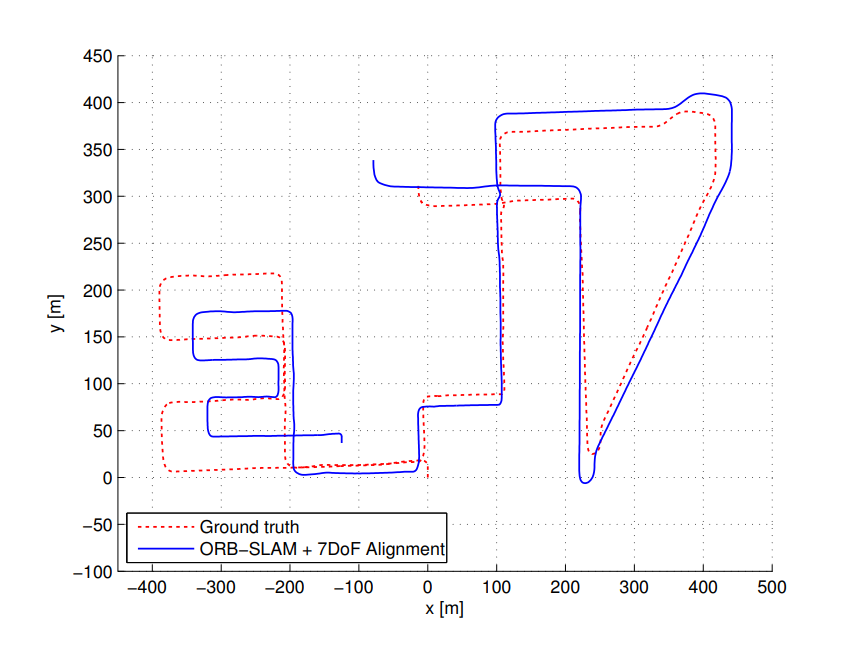
\includegraphics[width=0.4\textwidth]{Reports/3-Analysis-of-Baselines/images/orb08.png} % Replace with your image file
        \label{fig:orb-slam13}
    }
    \hspace{0.05\textwidth} % Space between subfigures
    \subfigure[Sequence 10]{
        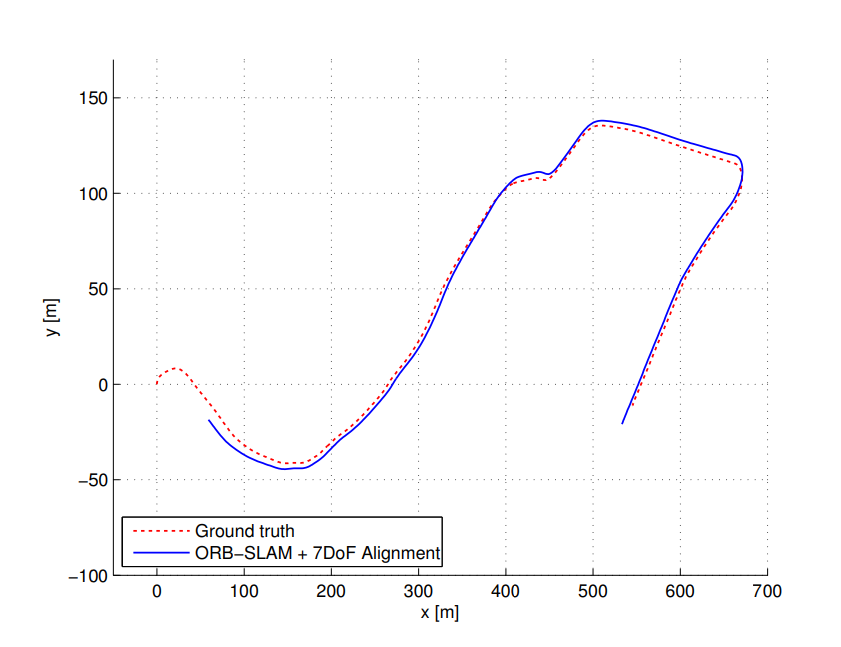
\includegraphics[width=0.4\textwidth]{Reports/3-Analysis-of-Baselines/images/orb10.png} % Replace with your image file
        \label{fig:orb-slam14}
    }
    \caption{Results of ORB-SLAM2 on KITTI Sequences 02, 08, 10. It is interesting to note the performances around loop crossings and long-tail trackings.}
    \label{fig:orb-slam2}
\end{figure}

\subsubsection{TartanVO}

TartanVO \cite{tartanvo} is the closest unimodal baseline to our work, as it uses the same two-frame formulation for odometry and is trained on the same dataset we plan to use, TartanAir \cite{tartanair}. It also uses optical flow to establish correspondences between frames for pose estimation. Our goal is to match or exceed TartanVO’s performance when trained on only image data, and with the addition of LiDAR data, the performance should improve significantly as LiDAR provides crucial information, enabling 3D grounding and more accurate pose estimation.

The intrinsic metric we want to test against for TartanVO is their flow loss. Since we also plan on using flow as a method or correspondence computation, we analyze the effects of learning from a flow pre trained flow model, GMFlow, and how this affects the motion prediction.

\begin{figure}[htbp]
    \centering
    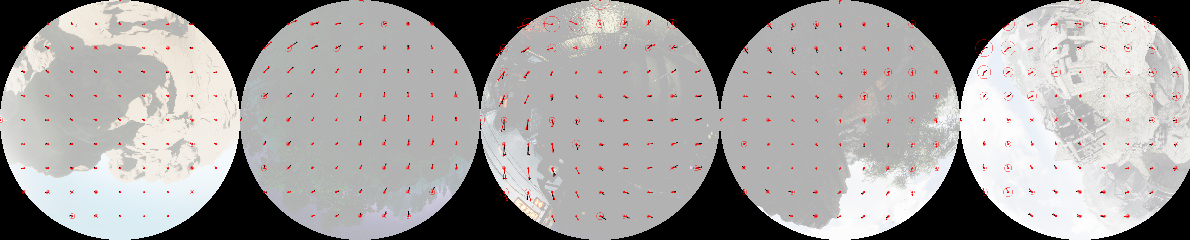
\includegraphics[width=8cm]{Reports/3-Analysis-of-Baselines/images/tartanvo/flow_img.png}
    \caption{Example intermediate flow visualizations from TartanVO}
    \label{fig:tvo-flow-img}
\end{figure}

\begin{figure}[htbp]
    \centering
    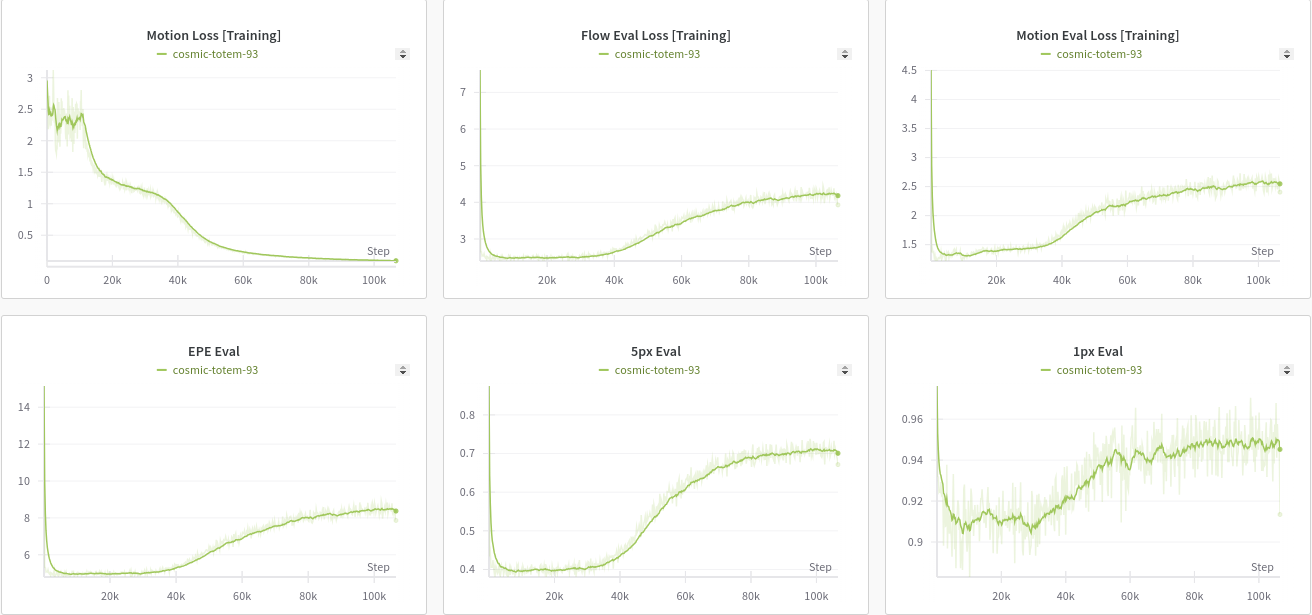
\includegraphics[width=8cm]{Reports/3-Analysis-of-Baselines/images/tartanvo/flow_loss.png}
    \caption{TartanVO motion and flow metrics during validation}
    \label{fig:tvo-flow-loss}
\end{figure}

\begin{figure}[htbp]
    \centering
    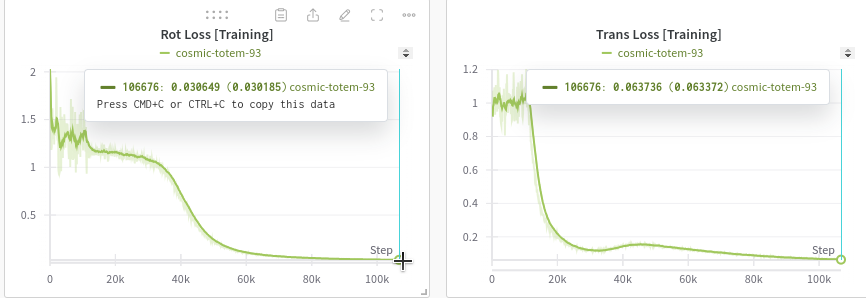
\includegraphics[width=8cm]{Reports/3-Analysis-of-Baselines/images/tartanvo/rot_trans_loss.png}
    \caption{TartanVO motion losses for rotation and translation}
    \label{fig:tvo-rot-trans}
\end{figure}

As shown in Figure \ref{fig:tvo-flow-loss}, we see that flow has an interesting relationship with the overall motion loss. The model is initialized with pre-trained flow and is trained using MSE on the motion. We see in the first plot that training motion loss starts off small and decreases, and in the second plot the flow validation loss starts off small, and in the third plot, the motion validation plot starts off small. This shows that flow can be a strong inductive bias to initialize odometry. More interestingly, as training progresses and the model overfits, we see that the training motion loss decreases while the validation motion and flow losses increase, showing that there is a tight correlation between the model's ability to perform optical flow and its ability to predict pose.

Another test we wanted to do with TartanVO is checking the scales of the rotation and translation components of the loss. The overall training objective in the sum of the rotation and translation losses and, as shown in Figure \ref{fig:tvo-rot-trans}, the rotation loss seems to be lower than the translation. We will need to balance these two losses properly to achieve better performance, or the model will be biased toward learning rotations over translations.

\subsection{LiDAR Odometry Methods}
We evaluated two LiDAR odometry methods: a classical approach, which is a variant of ICP SLAM that utilizes ScanContext for loop detection and miniSAM for loop closure, and a learning-based method, EfficientLO-Net \cite{eff-lo-net}. The evaluations of both methods are presented in the following sub-sections. 

\subsubsection{ICP-SLAM}
A SLAM pipeline, evaluated using only poses as states, was tested with ICP SLAM for odometry, Scan Context for loop detection, and miniSAM-based graph optimization on the KITTI dataset. The entire trajectory was empirically assessed to understand the pipeline's performance. For ICP, random downsampling with 7000 points was used, while the parameters for Scan Context were set to: Ring = 20, Sector = 60, and 30 ring key candidates. 

Figure \ref{fig:icp-kitti-2} illustrates the pipeline's performance on KITTI trajectory 2, with a loop closure threshold of 0.11. In this case, the loop was correctly detected, and the trajectory was optimized, aligning with the expected performance. Figures \ref{fig:icp-kitti-8} show the performance on KITTI trajectory 8 with loop detection thresholds of 0.07 and 0.20, respectively. In this case, either no loop was detected or a false loop was identified. This suggests that Scan Context may struggle with loop detection in scenarios where there is a significant change in lane level, as observed in KITTI trajectory 8.

\begin{figure}[htbp]
    \centering
    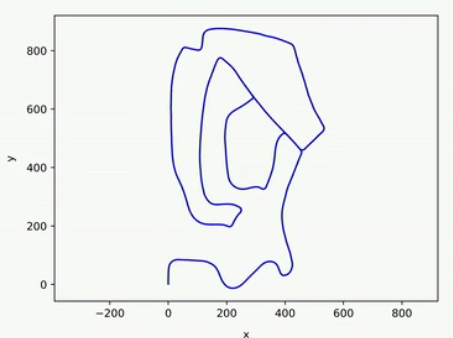
\includegraphics[width=4cm]{Reports/3-Analysis-of-Baselines/images/ICP-SLAM/KITTI_loop2.png}
    \caption{ICP SLAM on Trajectory 2: Loop Detected}
    \label{fig:icp-kitti-2}
\end{figure}

\begin{figure}[htbp]
    \centering
    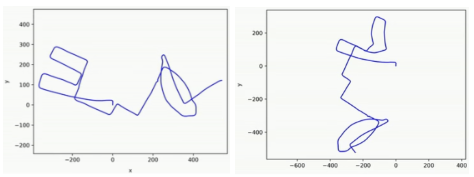
\includegraphics[width=8cm]{Reports/3-Analysis-of-Baselines/images/ICP-SLAM/kitti-08.png}
    \caption{ICP SLAM on Trajectory 8: Left - Threshold 0.007, Right - Threshold 0.20}
    \label{fig:icp-kitti-8}
\end{figure}

\subsubsection{EfficientLO-Net}
Efficient LO-Net was evaluated as a learning-based lidar odometry method. The average translational error(\%) for sequences 00-05, over distances ranging from 100 to 800 meters, remained below 0.55\%, with the rotational error (deg/m) not exceeding 0.38. In contrast, for Sequence 08, the translational error increased to 1.14\%. Sequence 08 presents a particularly challenging urban environment, characterized by sharp turns, intersections, dynamic obstacles like moving vehicles, and varying road structures. These elements likely posed significant challenges for Efficient LO-Net, making it difficult to maintain accurate feature associations across frames. The presence of dynamic objects and the complex structure of the scene likely contributed to increased translational drift, as the model may have struggled to differentiate between the vehicle’s motion and that of surrounding objects and to manage occlusions and variable feature distributions in the lidar data.



\begin{figure}[t]
\centering
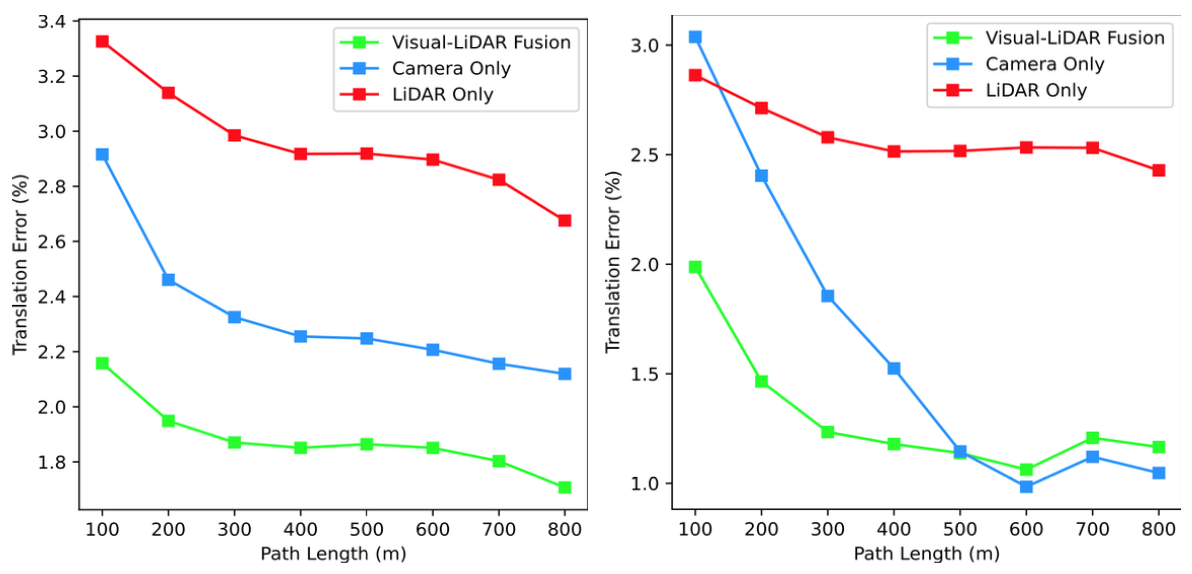
\includegraphics[width=\columnwidth]{Reports/3-Analysis-of-Baselines/images/HVLO-ablations.png}
\caption{
    Translation errors averaged across sub-sequences of various lengths (100, 200, ..., 800 meters) within sequences 09 and 10 of the KITTI dataset. The performance results for the LiDAR-only method (red lines), camera-only method (blue lines), and LiDAR-camera fusion method (green lines) are displayed.
}
\vspace{-0.4cm}
\label{fig:multimodal-plot}
\end{figure}
\begin{figure}[t]
\centering
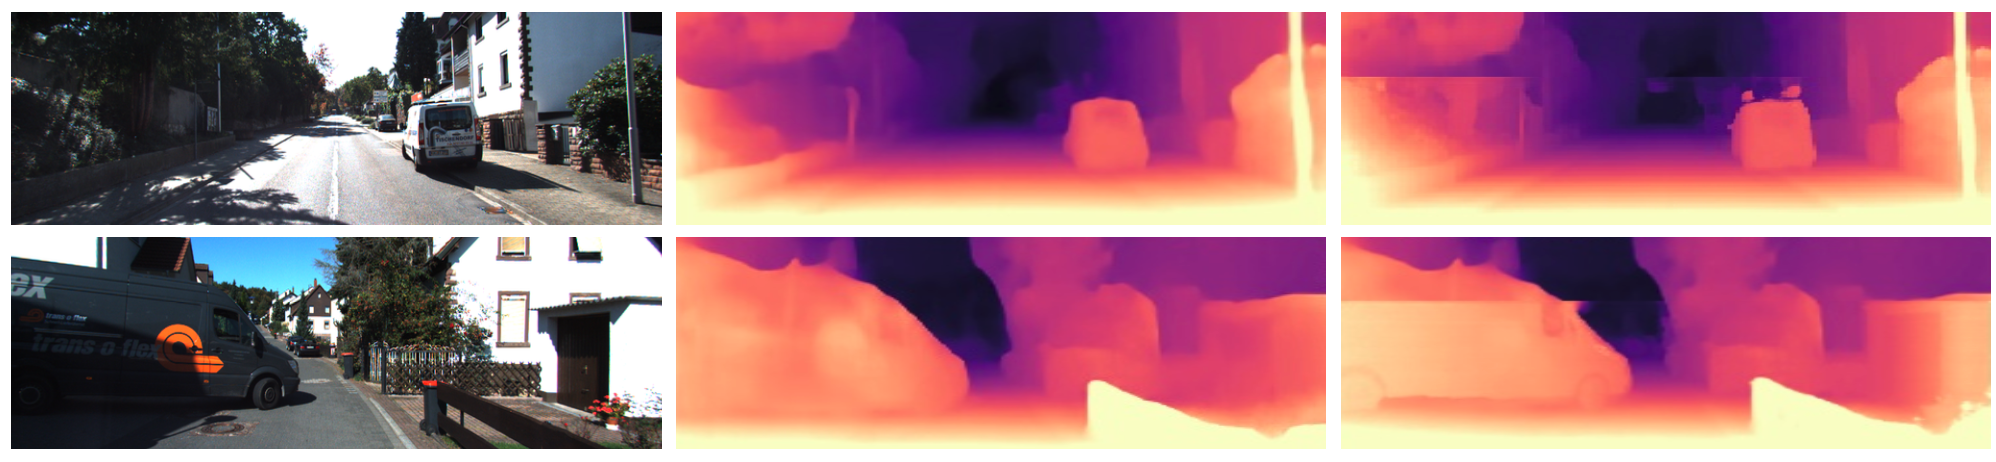
\includegraphics[width=\columnwidth]{Reports/3-Analysis-of-Baselines/images/HVLO-ablations-pic.png}
\caption{
    Effectiveness of visual-LiDAR fusion for better estimation of dense depth map. Each row contains one example of the improvement in RGB image frame, DepthNet estimation, fusion result, respectively. Top row: attachments to the roof of the vehicle exist in the fused map where DepthNet is not able to estimate it. Bottom row: Vehicle boundaries are more noticeable and DepthNet is fooled due to graphics at the side hood of the van.
}
\vspace{-0.4cm}
\label{fig:multimodal-pic}
\end{figure}

\subsection{Multimodal Odometry Methods}

\subsubsection{H-VLO}
Since H-VLO~\cite{hvlo} demonstrates robust performance by effectively combining LiDAR and camera modalities, we leverage its structure to examine the benefits of integrating these modalities in a LiDAR-camera fusion method. This approach is contrasted with single-modality methods that rely solely on either LiDAR or camera data, allowing us to isolate and understand the unique advantages provided by each data source as well as their combined effect. Figure~\ref{fig:multimodal-plot} illustrates the translational errors averaged across sub-sequences of various lengths (100, 200, ..., 800 meters) within sequences 09 and 10 of the KITTI dataset. The performance results for the LiDAR-only method (red lines), camera-only method (blue lines), and LiDAR-camera fusion method (green lines) are displayed.

The LiDAR-only method, represented by the red lines, yields the least accurate trajectory estimates, showing that depth information alone is insufficient for precise motion estimation and mapping, particularly in scenarios where detailed semantic cues are essential for distinguishing objects and understanding scene context. Without these semantic details, the LiDAR-only approach struggles, resulting in higher translational errors, particularly over longer sub-sequence lengths.

On the other hand, the camera-only method (blue lines) performs notably better, benefiting from the rich semantic information inherent in RGB images. Camera data captures texture, color, and object detail, which enhances scene interpretation and aids in predicting object movements and scene transitions. As a result, the camera-only method achieves significantly lower translational errors compared to the LiDAR-only approach, especially in sub-sequences where scene complexity demands higher contextual understanding. However, despite its advantages, the camera-only method still encounters limitations in environments where depth perception is crucial but cannot be accurately derived from monocular RGB images alone.

By combining the semantic information from camera data with the depth and structural detail from LiDAR data, the LiDAR-camera fusion approach (green lines) harnesses the strengths of both modalities. This fusion achieves superior results by providing a more comprehensive representation of the environment: LiDAR contributes precise spatial geometry, while the camera supplies detailed scene semantics. Leveraging the fusion structure within H-VLO, the LiDAR-camera fusion method demonstrates the lowest translational errors across all sub-sequence lengths, suggesting that integrating these complementary data sources not only improves trajectory accuracy but also enhances robustness in complex environments with varying levels of occlusion, lighting, and scene intricacies.

\subsubsection{DVLO}
Most learning-based approaches, such as H-VLO~\cite{hvlo}, focus on feature-level fusion but often fail to capture the fine-grained pixel-to-point correspondences required for precise pose estimation. These approaches are further challenged by the inherent structural differences between sparse LiDAR points and dense camera pixels, resulting in data misalignment that limits the effectiveness of multi-modal fusion.

To address these limitations, DVLO~\cite{dvlo} introduces a novel local-to-global fusion network with bi-directional structure alignment, specifically designed to enhance the integration of LiDAR and visual features for more accurate pose estimation. In particular, DVLO clusters neighboring visual information in 2D images by projecting LiDAR depth data onto the 2D image plane. This clustering enables effective alignment of LiDAR points with visually similar pixels, improving spatial consistency.

As shown in Figure~\ref{fig:dvlo}, pixels with similar texture information (yellow regions) are clustered by calculating the point-wise cosine similarity with designated cluster centers (red dots). This approach ensures that visual information is more cohesively grouped with corresponding depth data, leading to a more refined fusion of LiDAR and visual features and ultimately resulting in enhanced pose estimation accuracy.

\begin{figure}[htbp]
    \centering
    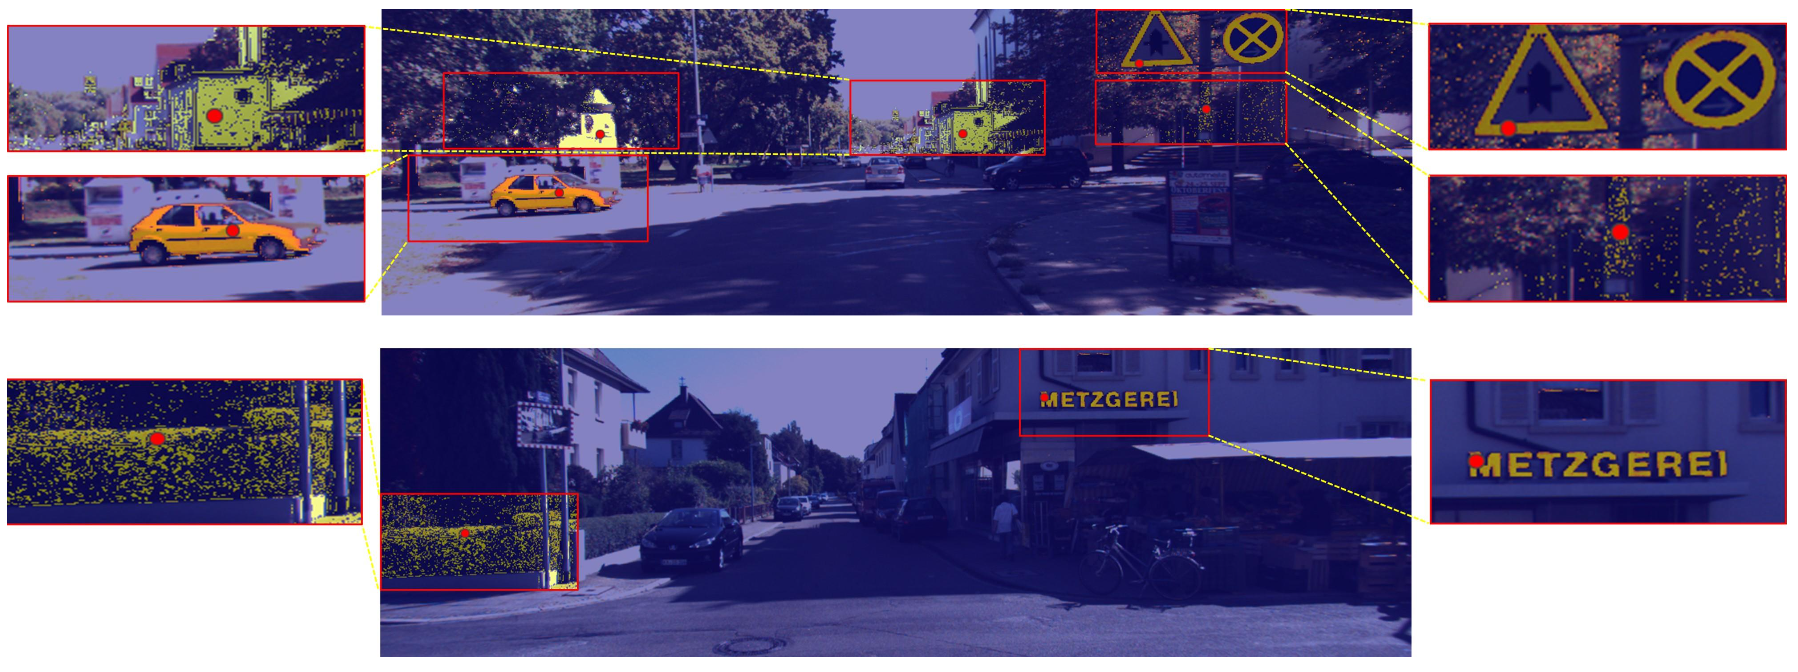
\includegraphics[width=8cm]{Reports/3-Analysis-of-Baselines/images/dvlo.png}
    \caption{Visualization of DVLO's local clustering-based fusion mechanism within a certain cluster. Red points indicate the 2D positions of cluster centers. The yellow regions are clustered pixels around each center.}
    \label{fig:dvlo}
\end{figure}

\subsubsection{SDV-LOAM}
SDV-LOAM (Semi-Direct Visual-LiDAR Odometry and Mapping) \cite{sdv-loam} was evaluated as one of the classical multimodal baselines. It is a robust odometry method that effectively combines visual and LiDAR data for accurate pose estimation and mapping. The system addresses common challenges in visual-LiDAR fusion by incorporating a semi-direct visual odometry approach and an adaptive sweep-to-map LiDAR odometry.

The visual module of SDV-LOAM employs a novel technique that directly extracts high-gradient pixels where 3D LiDAR points project for tracking, avoiding the need for explicit 3D-2D depth association. To handle large-scale differences between matching frames, it uses a point matching with propagation method, which propagates points from a host frame to an intermediate keyframe closer to the current frame. This approach significantly reduces scale differences and improves tracking accuracy.

On the LiDAR side, SDV-LOAM introduces an adaptive sweep-to-map optimization method that dynamically chooses between optimizing 3 horizontal degrees of freedom (DOF) or 6 full DOF pose based on the richness of geometric constraints in the vertical direction. This adaptive approach helps reduce pose estimation drifts, particularly in the vertical direction. Some interesting results of the interesting inference runs are shown in figure \ref{fig:sdv-loam}.

\begin{figure}[h!]
    \centering
    \subfigure[Sequence 13]{
        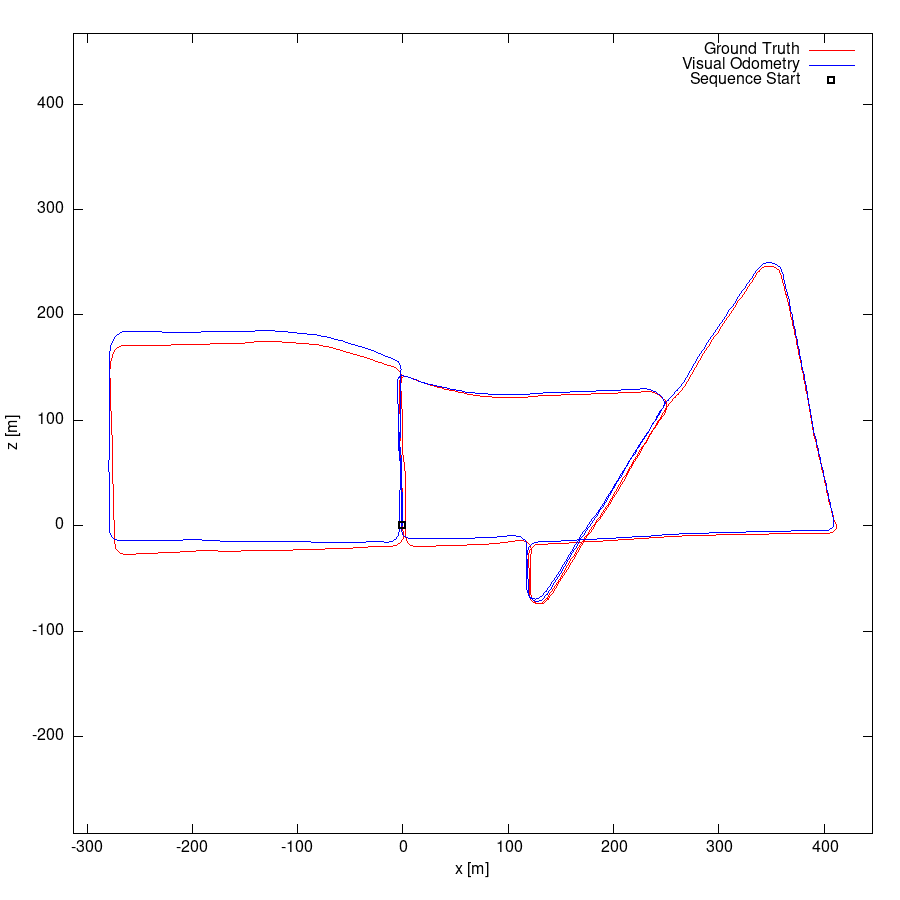
\includegraphics[width=0.4\textwidth]{Reports/3-Analysis-of-Baselines/images/sdv13.png} % Replace with your image file
        \label{fig:sdv13}
    }
    \hspace{0.05\textwidth} % Space between subfigures
    \subfigure[Sequence 14]{
        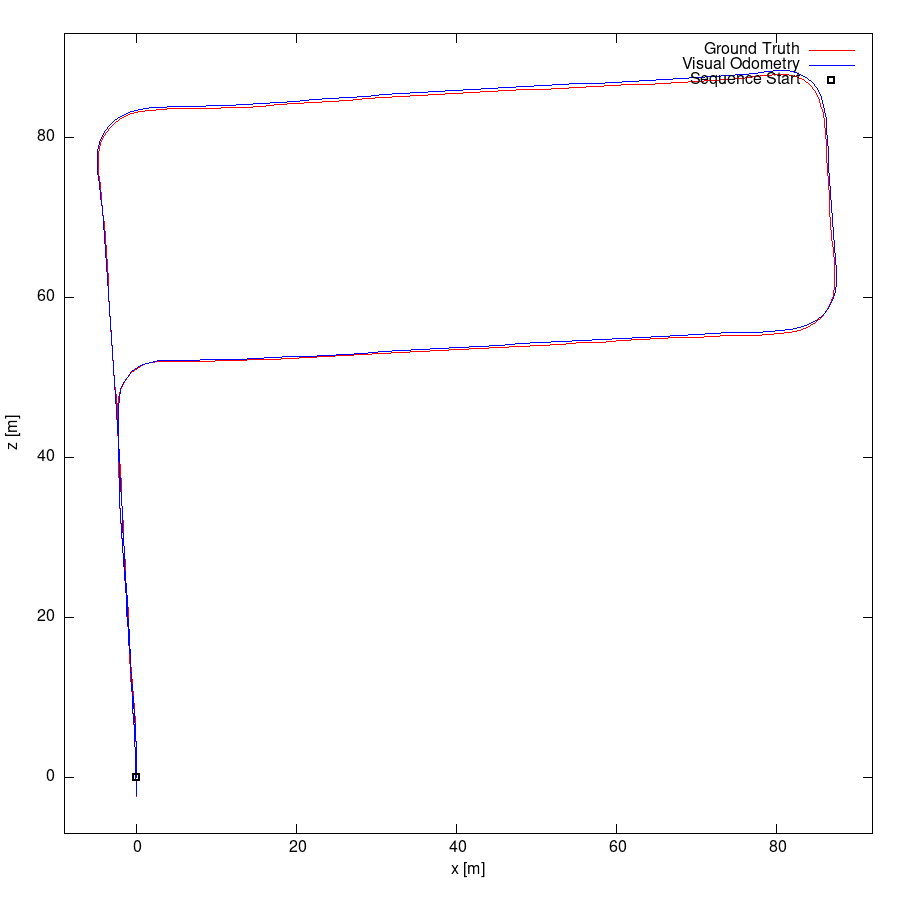
\includegraphics[width=0.4\textwidth]{Reports/3-Analysis-of-Baselines/images/sdv14.png} % Replace with your image file
        \label{fig:sdv14}
    }
    \hspace{0.05\textwidth} % Space between subfigures
    \subfigure[Sequence 15]{
        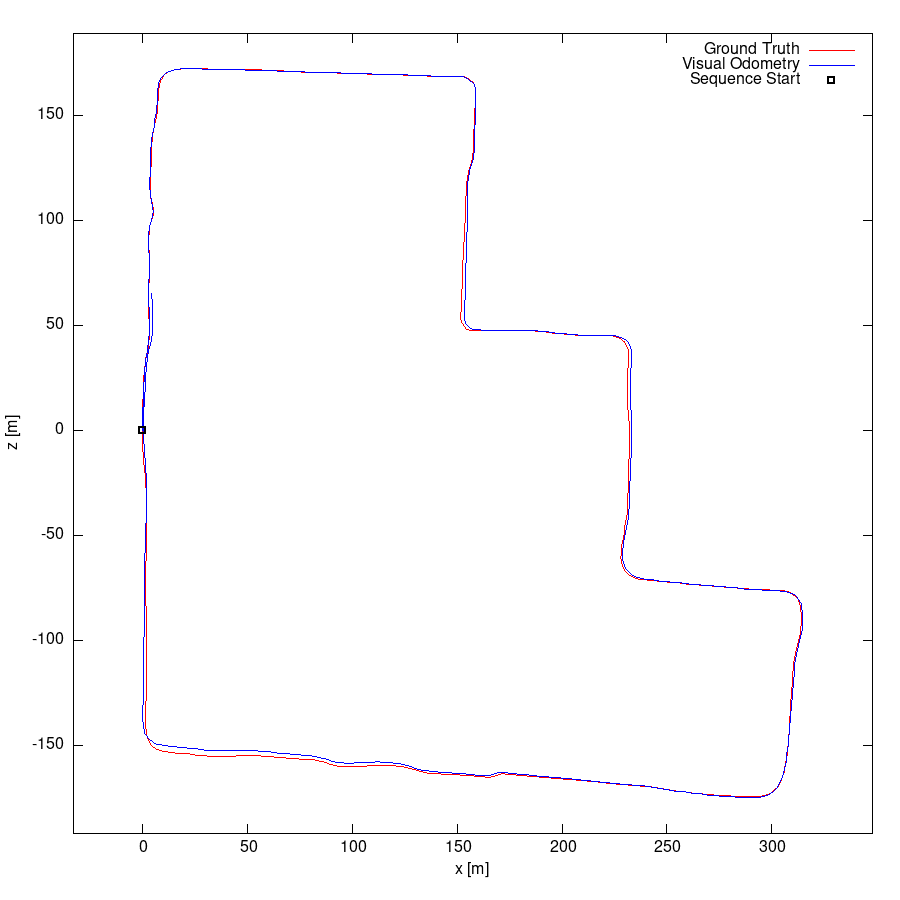
\includegraphics[width=0.4\textwidth]{Reports/3-Analysis-of-Baselines/images/sdv15.png} % Replace with your image file
        \label{fig:sdv15}
    }
    \caption{Results of SDV-LOAM on KITTI Sequences 13, 14, 15 \cite{KITTI}.}
    \label{fig:sdv-loam}
\end{figure}





% % Update this table with your extrinsic and intrinsic metrics.  
% % Update rows with what you ran
% % How well did they do on every metric?
% \begin{table}[t]
% \centering
% \begin{tabular}{@{}lrr@{}}
% \toprule
%                             & \multicolumn{2}{c}{Dev} \\
% Methods                     & Detections $\uparrow$ & Invalid Actions $\downarrow$  \\
% \midrule
% Unimodal 1 \cite{} & & \\
% Unimodal 2 \cite{} & & \\
% Unimodal 3 \cite{} & & \\
% \midrule
% Simple Multimodal 1 \cite{} & &  \\
% Simple Multimodal 2 \cite{} & &  \\
% Simple Multimodal 3 \cite{} & &  \\
% \midrule
% Previous Approach 1 \cite{} & &  \\
% Previous Approach 2 \cite{} & &  \\
% Previous Approach 3 \cite{} & &  \\
% \bottomrule
% \end{tabular}
% \end{table}

% \begin{table*}[t]
  \centering
  \caption{Comparison with different odometry networks on the KITTI odometry dataset. $t_{rel}$ and $r_{rel}$ mean the average sequence translational RMSE (\%) and the average sequence rotational RMSE ($^{\circ}$/100m) respectively on 06, 07, 09, 10 subsequences.\\ (*) Means learning based methods, whereas (-) means classical methods.} 

    \begin{tabular}{lllll|cc|cc|cc|cc}
    \toprule
    \multicolumn{5}{l|}{\multirow{2}[0]{*}{\textbf{Method}}} & \multicolumn{2}{c|}{06} & \multicolumn{2}{c|}{07} & \multicolumn{2}{c|}{09} & \multicolumn{2}{c}{10} \\
         &      &      &      &      & $t_{rel}$ & $r_{rel}$ & $t_{rel}$ & $r_{rel}$ & $t_{rel}$ & $r_{rel}$ & $t_{rel}$ & $r_{rel}$\\
    \midrule
    \multicolumn{13}{l}{\it{Visual Odometry Methods:}} \\
    \midrule
    \multicolumn{5}{l|}{ORB-SLAM (-)} & 18.68 & 0.26 & 10.96 & 0.37 & 15.3 & \textbf{0.26} & 3.71 & \textbf{0.3}  \\
    \multicolumn{5}{l|}{TartanVO (*)} & 4.72 & 2.95 & 4.32 & 3.41 & 6.0 & 3.11 & 6.89 & 2.73 \\
    \midrule
    \multicolumn{13}{l}{\it{LiDAR Odometry Methods:}} \\
    \midrule
    \multicolumn{5}{l|}{ICP-SLAM (-)} & 1.95 & 1.59 & 5.17 & 3.35 & 6.93 & 2.89 & 8.91 & 4.74  \\
    \multicolumn{5}{l|}{LO-Net (*)} & 1.04 & 0.69 & 0.71 & 0.50 & 2.12 & 0.77 & 1.80 & 0.93 \\
    \midrule
    \multicolumn{13}{l}{\it{Multimodal Odometry Methods:}} \\
    \midrule
    \multicolumn{5}{l|}{H-VLO (*)} & 0.75 & 0.30 & 0.79 & 0.48 & 1.89 & 0.34 & 1.36 & 0.43 \\
    \multicolumn{5}{l|}{DVLO (*)} & \textbf{0.33} & \textbf{0.17} & \textbf{0.46} & \textbf{0.33} & 0.85 & 0.36 & 0.88 & 0.46 \\
    \multicolumn{5}{l|}{DV-LOAM (-)} & 0.65 & 0.33 & 0.51 & \textbf{0.33} & 0.73 & 0.32 & 0.87 & 0.38 \\
    \multicolumn{5}{l|}{SDV-LOAM (-)} & 0.50 & 0.27 & 0.84 & 0.53 & \textbf{0.63} & 0.34 & \textbf{0.68} & 0.41 \\
    % \midrule
    
    \bottomrule
    \end{tabular}%
  \label{tab:evaluation_06_10}%
\end{table*}


% \clearpage
\subsection{Qualitative Analysis and Examples}

\begin{figure}[h!]
    \centering
    \subfigure[ORB-SLAM2]{
        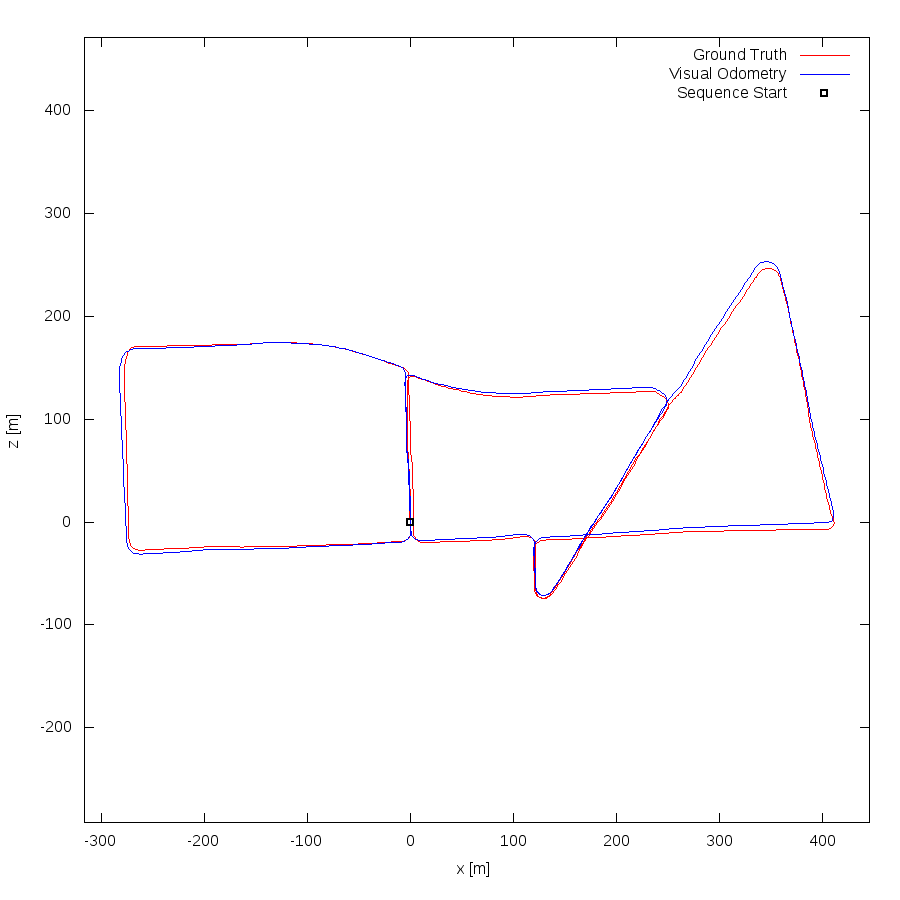
\includegraphics[width=0.3\textwidth]{Reports/3-Analysis-of-Baselines/images/orb.png} % Replace with your image file
        \label{fig:orbslam13}
    }
    \subfigure[DVLO]{
        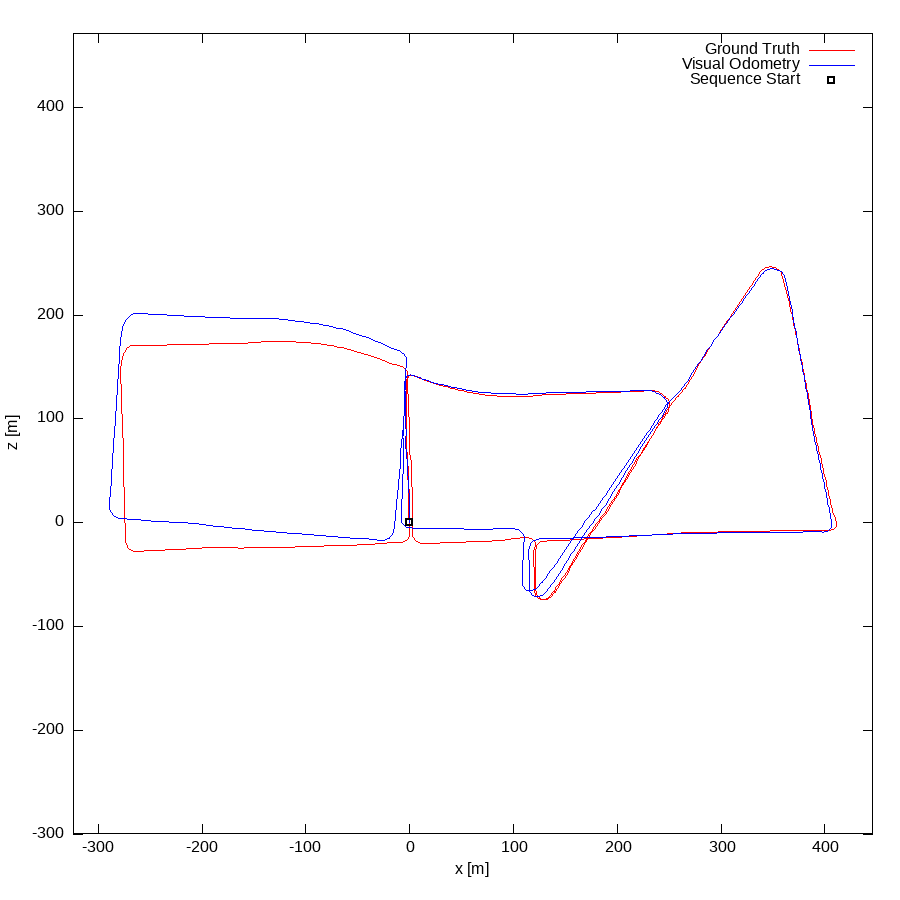
\includegraphics[width=0.3\textwidth]{Reports/3-Analysis-of-Baselines/images/dvlo13.png} % Replace with your image file
        \label{fig:dvlo13}
    }
    \hspace{0.05\textwidth} % Space between subfigures
    \subfigure[EfficientLO-Net]{
        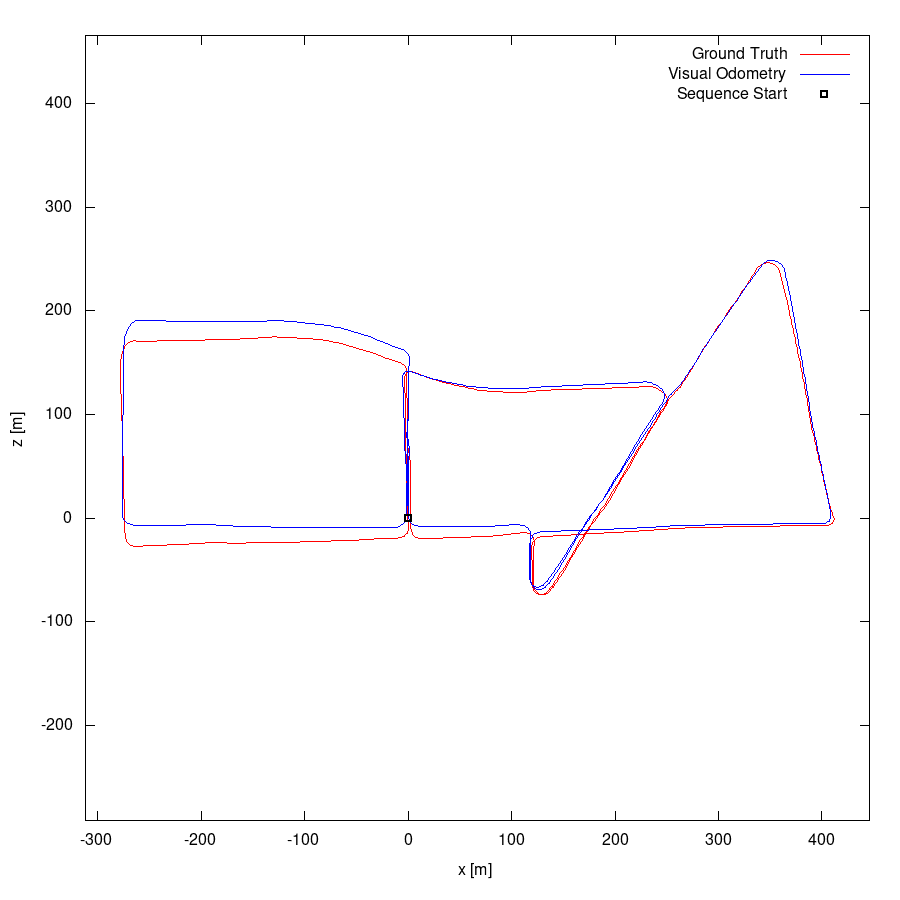
\includegraphics[width=0.3\textwidth]{Reports/3-Analysis-of-Baselines/images/lonet13.png} % Replace with your image file
        \label{fig:lonet13}
    }
    \hspace{0.05\textwidth} % Space between subfigures
    \subfigure[SDV-LOAM]{
        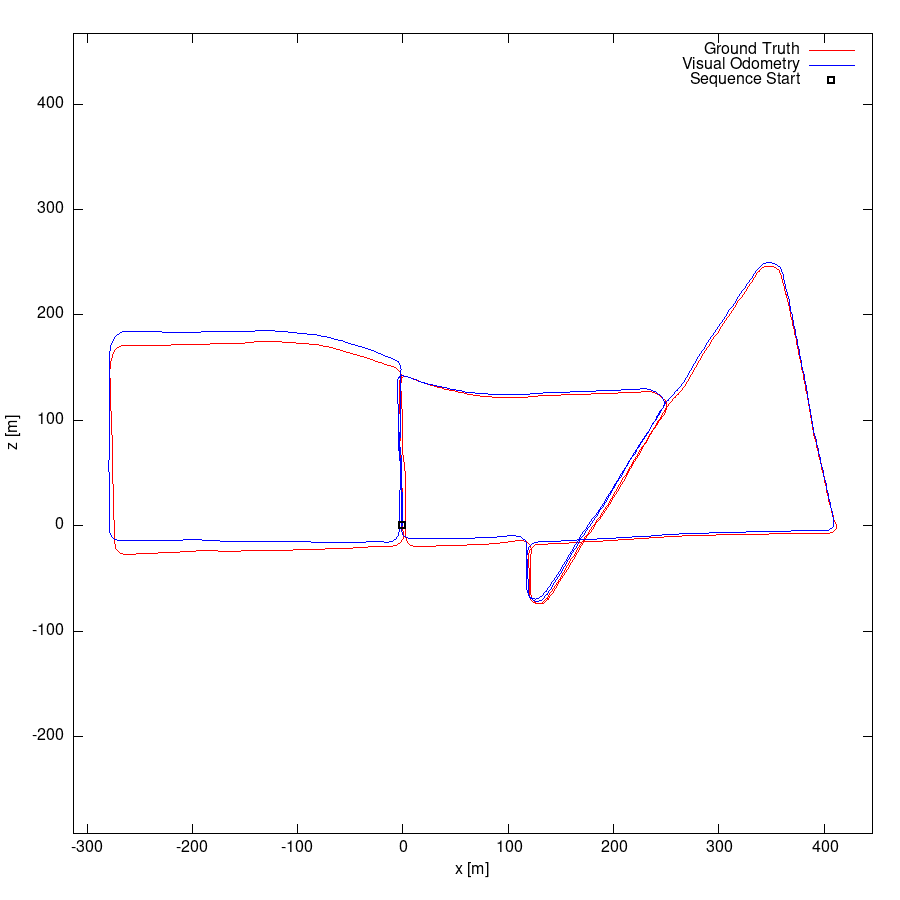
\includegraphics[width=0.3\textwidth]{Reports/3-Analysis-of-Baselines/images/sdv13.png} % Replace with your image file
        \label{fig:sdv13}
    }
    \caption{Results of ORB-SLAM2, EfficientLO-Net, DVLO, SDV-LOAM on KITTI Sequence 13.}
    \label{fig:seq13}
\end{figure}



\paragraph{Insights}
% Two paragraphs on what you found and how they impact your expectations for the main model, or how they have inspired you to change your proposed approach, etc

Our analysis of the baseline models individually in the previous section highlighted that each modality has distinct strengths—LiDAR excels in spatial precision, while RGB provides critical semantic context. However, each also shows limitations: LiDAR alone leads to higher translational errors due to lacking semantic cues, and RGB struggles with scale ambiguity. These findings confirm the value of multimodal fusion, motivating us to refine our model to more effectively integrate depth and semantic information. 

We report the performances of select baseline models on the same KITTI scene in Figure \ref{fig:seq13}. Notice that each model has slightly different failure modes and performances. ORB-SLAM has the best performance as it is a well tested classical model, however it also has loop closure and takes much longer to process. It's failure mode is real-time setting. Also, some turns, such as the one on the top right with large motions, are a little imprecise. DVLO performs a little better on that turn as it is a leanring based model and has strong priors. However, it accumulates drigt on long straight paths, similar to EfficientLO-Net. This seems to be a general problem with learning-based models. SDV-LOAM corrects this drift using its LiDAR processing, however it is still not completely solved. Overall, it seems all learning-based models have large drift problems.

The strong performance of multimodal baselines like H-VLO~\cite{hvlo} has further inspired us to enhance our cross-attention mechanism with adaptive weighting. By dynamically adjusting each modality’s influence based on scene context, our model can better prioritize LiDAR in geometric tasks and RGB in semantic-rich settings. This adjustment is expected to improve both accuracy and robustness across diverse scenarios.

The learning-based lidar odometry model, EfficientLO-Net, faced challenges with sequence 12 due to the complexity of the environment, dynamic obstacles, and occlusions. These factors made it difficult for the model to reliably associate features across frames and maintain accurate motion estimates. As shown in Figure \ref{fig:lo-net}, the comparison between the ground truth trajectory and the estimated trajectory reveals significant drift.


\begin{figure}
    \centering
    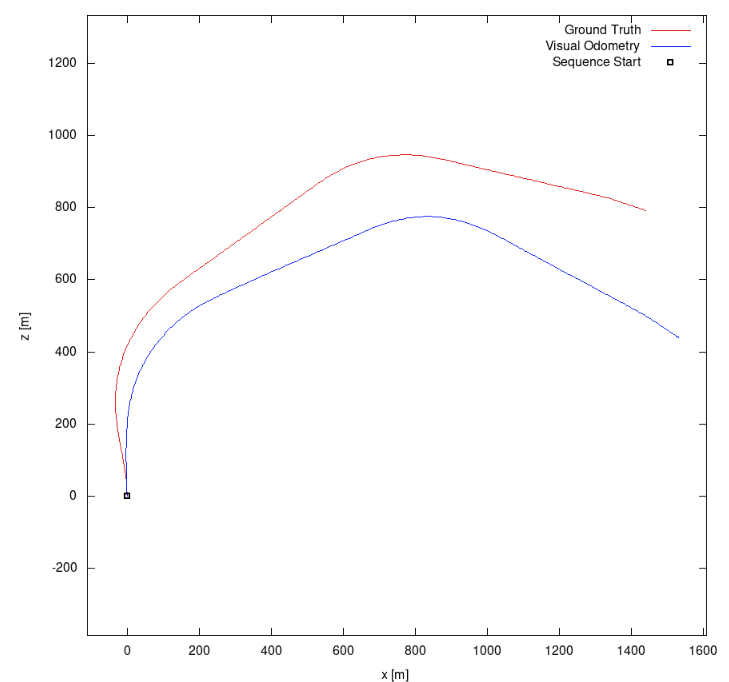
\includegraphics[width=5cm]{Reports/3-Analysis-of-Baselines/images/Efficeint_Lonet.png}
    \caption{EfficientLO-Net on KITTI Sequence 12}
    \label{fig:lo-net}
\end{figure}
 

% \clearpage
\section{Team member contributions}
\paragraph{Pujith Kachana} contributed to evaluation results and metric on TantanVO and other baselines as well as insights ans synthesis.

\paragraph{Yatharth Ahuja} contributed to exploring and evaluating unimodal baselines, and in the qualitative analysis.

\paragraph{Shashwat} contributed to exploring and evaluating unimodal baselines, and in the qualitative analysis.

\paragraph{Ming Feng Li} contributed to evaluating and analyzing multimodal methods that combine RGB and LiDAR modalities.

% Please use 
\bibliographystyle{acl_natbib}
\bibliography{references}

%\appendix



\end{document}
